% Chapter Template

\chapter{ Medical Imaging} % Main chapter title

\label{Chapter2} % Change X to a consecutive number; for referencing this chapter elsewhere, use \ref{ChapterX}
 
 %----------------------------------------------------
 
 
Radiology gave to the physician a look of the inside the human body without the need for surgery. Images diagnostics has evolved over time, with the introduction of new imaging tools, protocols and imaging technologies based on the use of ionizing radiation and other physical principles. The current diagnostic equipment are accurate, smaller and emits less radiation than before . Moreover, the most recent tools allow to acquire diagnostic data in digital form, enabling data post-processing using dedicated software. Diagnostic images have gone from having only a diagnostic function to being often the basis for the treatment planning.
At the basis of modern digital diagnostics is the \textbf{DICOM} standard (\emph{\textbf{D}igital \textbf{I}maging and \textbf{CO}munication in \textbf{M}edicine}). The standard is freely available online, it can be freely used \parencite{Reference27}. On this Standard is based the whole chain of modern patient management, from the acquisition of clinical and anamnestic data to diagnostic images, up to the transfer of data between different health workers \parencite{Reference25}.

\section{Scanning of the human body}
The human organism is a three-dimensional object oriented in space. In anatomy we describe the human organism located in the \emph{Anatomical Position}.\\
Scanning of the human organism can be performed with different techniques and tools. The scan can represent only the surface of the organism, or also capture its internal organs.

\subsection{Computer Tomography}
Computer Tomography (CT) is a technique that uses beams of X-rays that pass through the human body and are detected by a scanner, that evaluate the energy absorbed during the path, and therefore the density of the tissues (in Hunsfield Unit). This measurement is performed from various angles on the same plane, and the readings are processed by software, which returns an image that is a map of the density of the scanned organism (\emph{\textbf{slice}}). \\
The image is a grid of \textbf{voxel} (whose resolution depends on various factors, including the device used and the FOV (\emph{Field Of View}), always according to the \emph{ALARA} principle), in which each voxel is represented in a shade of gray proportional to the attenuation of the X ray, by the tissue founded in the represented volume. The slices are acquired, one after the other, at a thickness (\emph{slice thickness}) and a distance (\emph{pitch}, \parencite{Reference23}) that depend on the used tomograph and the implemented scanning protocol. The slices acquired are then ordered to form a images series, and each slice is interpolated with the subsequent, allowing to obtain a real volume.
The volume thus constituted can be studied on arbitrary planes of space, thanks to \emph{multiplanar reconstruction algorithms} (MRP). The volumetric representation thus created is of great importance, because it is the base of modern radiological diagnosis and therapy.

\subsection{Cone Beam Computer Tomography (CBCT)}
CBCT is a technique that uses the same physical principles as CT, but presents differences due to scan procedure and reconstruction algorithms \parencite{Reference12}, \parencite{Reference13}.\\
The CBCT scanner uses a conical beam of X-rays, which is rotated around the region to be scanned (\textbf{ROI} - \emph{region of interest}) and is detected by a sensor, placed orthogonal to the beam. The conical beam allows to acquire a volume during the revolution, so the scans are faster and with a lower dose of radiation absorbed by the patient than a conventional CT \parencite{Reference14}. \\
CBCT equipment is smaller and mechanically less complex than conventional CTs; these characteristics, associated with the scanning speed and the lower cost, have made it widespread, especially in the diagnostic of the oromaxillofacial region. The reduced FOV allows to reduce the absorption of radiation and to provide high resolution 3D reconstructions. Interesting is also the fact that these devices, given their small size, have been used as an intraoperative aid during surgery \parencite{Reference15} and during endodontic therapy procedures in selected cases \parencite{Reference16}. \\ 
The diagnostic images obtained from the CBCT scan is the result of a first processing step, which allow to map in a three-dimensional space the data collected by the detector \parencite{Reference11}. The images collected are processed with algorithms to reduce artifacts due to the scanning process. The scattering \emph{noise} is relevant in the unprocessed images, so it is reduced through an image blur process (\emph{blurring} or \emph{smoothing}), finding a compromise with the preservation of the spatial resolution of the images (which is higher at low levels of blur, ie. when the image is well defined, \emph{edge sharpening}). \\
Of relevance, especially in the implant surgery planning, is the assessment of bone quality in the implant site. Historically, bone density, measured in \emph{Hounsfield Unit} (HU), has been the most used parameter to describe bone quality. Today's CBCT scanners do not give Hounsfield's scale images, but in a \emph{gray scale} (Gray Value, GV) which is the representation of the attenuation of the X-ray signal by the tissues found in the path of the beam. \\ It was shown how the grayscale representation is dependent on the scanner used, as well as being highly variable even in the same device. Differences in the representation of the density can be highlighted between the central and the peripheral area of an image, both on the horizontal and vertical axis. To partially obviate to this problem, the scanner must be calibrated with test samples provided by the manufacturer; variability remains even after calibration \parencite{Reference17}, but is considered acceptable for normal procedures. However, the search for algorithms and techniques to reduce scanning artifacts is one of the fields in which innovations \parencite{Reference19} are most frequently presented.\\
CBCT scaning device use a lower slice-thickness than conventional CT, improving the representation of small details, as the endodontic canal.

\begin{figure}[h]
    \centering
    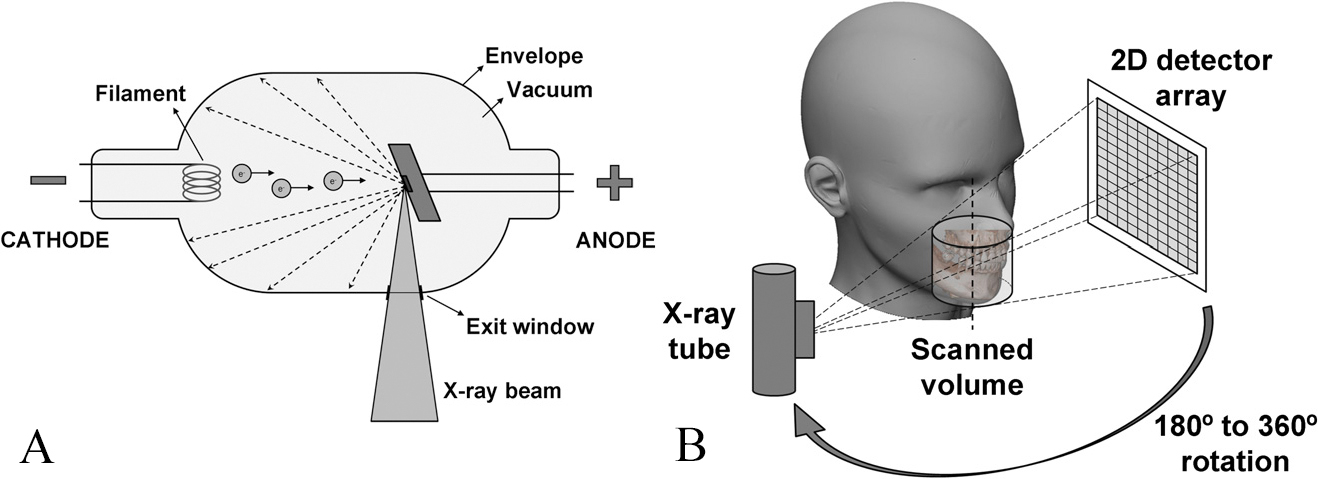
\includegraphics[width =\textwidth, height =\textheight, keepaspectratio]{cbct}
    \caption{\textbf{A}: simplified scheme of a \emph{X-ray tube}. The electric current heats the filament located at the cathode, leading to the release of electrons. The electrons are accelerated towards the anode by means of a potential difference. The collision of electrons on the target leads to the production of X-rays, which are emitted through the exit. The rays in other directions (dotted lines) are attenuated by the tube lining. \textbf{B}: we see the relationship between the X-Ray emitter and the detector, which are placed one in front of the other, and often joined by a C-arm. These two elements make a revolution around the region to be scanned, of an angle between 180 and 360 degrees. From Pauwels et al \parencite{Reference11}.}
    \label{fig: CBCT}
\end{figure}

\subsection{Magnetic Resonance}
Magnetic Resonance Imaging (MRI) uses magnetic fields to orientate water's molecules within the organism and to detect their position, through the energy emitted when they return to their initial configuration, after the magnetic field has been switched off. The scans are repeated to intensify the signal. The image obtained is in grayscale, with the richest areas of water showing a greater intensity (white) than areas with little water (black). MR equipment uses different parameters for detection, with protocols that allow to suppress or increase the signal intensity of a tissue.\\
MRI does not emit ionizing radiation, but it can be risky for the patient with metal implants or pacemakers, so these conditions must be assessed before subjecting the patient to the scan.\\
This imaging technique allows good visualization of the body's soft tissues, but bone margins are difficult to detect, especially at the level of alveolar processes. Some groups have however started to explore the potential of MRI also in the diagnosis of bone pathology \parencite{Reference18} and its microstructure \parencite{Reference19}
\begin{figure}[h]
    \centering
    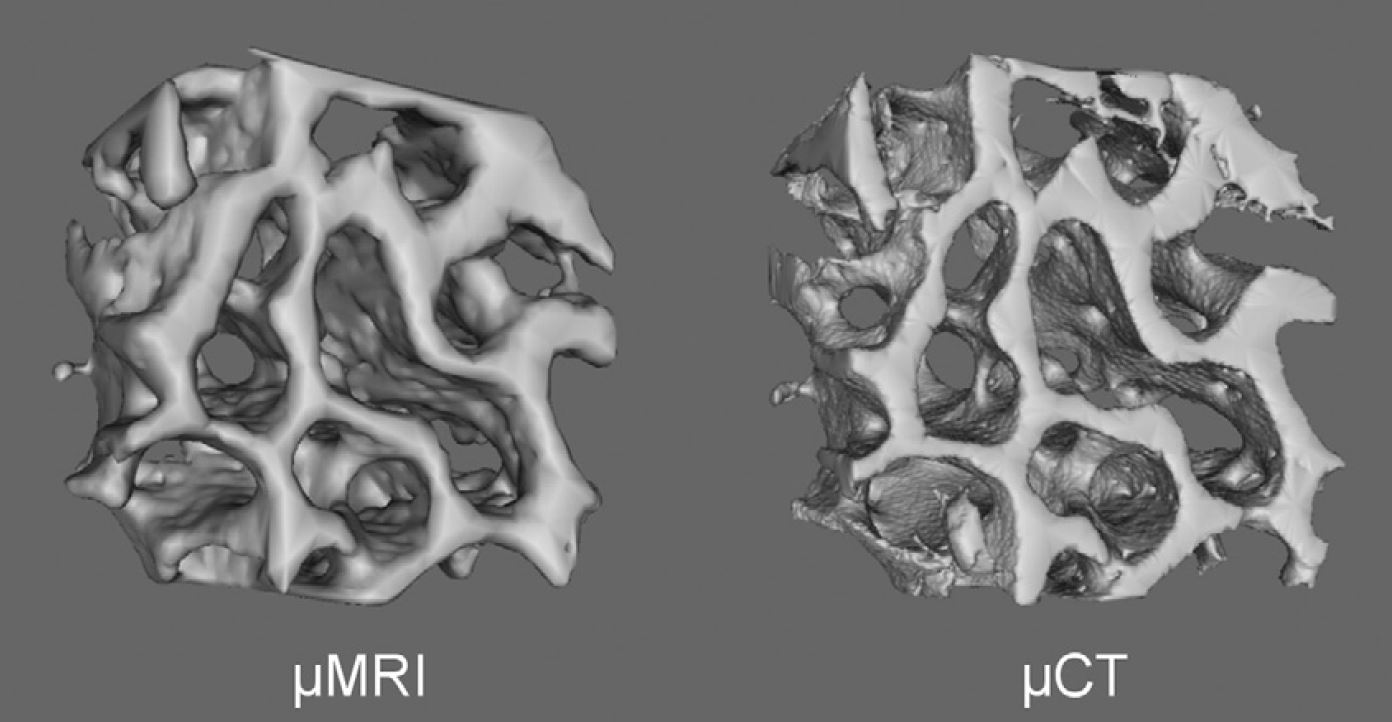
\includegraphics [width=0.5 \textwidth]{trabecole_CTvsMR} 
    \caption{reconstruction of bone trabeculation using two different imaging techniques. From Weiger et al \parencite{Reference19}.}
    \label{fig:trabeculae}
\end{figure}.

\subsection{Surface scans}
Surface scan makes possible to digitize the body surface and the cavities accessible by the scanning equipment.\\
In the dental field various optical scanning devices have spread, replacing the plaster impressions. These scanners allow to obtain digital impressions of the patient's arches, which are important for the subsequent therapy, that very often makes use of CAD/CAM devices for the design and manufacturing of temporary restoration and prosthesis.\\
There are several scanning technologies, but the most used in the medical field are techniques that reconstruct a three-dimensional surface starting from a series of images of the region to be digitized.\\
The instruments required for scanning usually consists of an image acquisition device, a computer and data processing software. The software assists the operator in the images acquisition, which are often processed in real time to provide the clinician with an instant view of the model being acquired. The three-dimensional model thus created can also contain the color of the scanned tissue (\emph{textures}) \parencite{Reference20}. \\
The acquired models can be used in combination with models made by CT or MRI, where the oral tissues are less defined than the models obtained with surface scanners, and may present artifacts due to the presence of prostheses or metal restorations, in addition to not having information of the surface textures. This combination allows the creation of high quality models to accurately plan orthognathic surgery procedures \parencite{Reference21}, \parencite{Reference22}. \\
Digital reconstructions of real objects can also be performed by means of a camera, with a technique called \emph{Photogrammetry}. This consists in acquiring a series of partially superimposed pictures around the object to be scanned; the images are then processed by algorithms to give a digital 3D model \parencite{Reference117}. \newpage
\begin{figure}[h]
\vspace{-10pt}
    \centering
    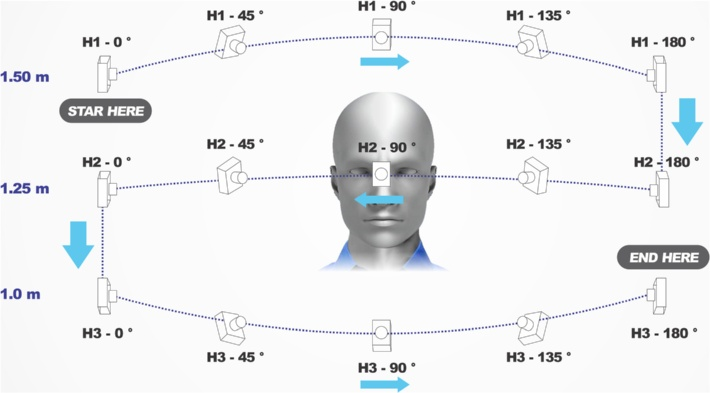
\includegraphics[width=0.8\textwidth, height=\textheight, keepaspectratio]{photogramm_capture}
    \caption{Photogrammetry protocol developed by Salazar-Gamarra et al \parencite{Reference117} for scanning a face using a mobile phone and 123D Catch software (now no longer active).}
    \label{fig:photogramm_capture}
\end{figure}

\section{Problems related to scans}
Digital images share the problem of \emph{\textbf{partial volume effect}}. It consists in the fact that a voxel can represent a single shade of gray, so if in the volume of a voxel there is more than one tissue, perhaps at different densities, the density represented in the voxel will be a weighted average of the densities present in the voxel volume. A decrease in the size of the voxels (and therefore an increase in the number of voxels with the same volume) makes it possible to partially compensate for the problem. \\ This problem is always to be taken into account during image segmentation, because it affects the quality of the details and the discrimination of the boundary of different tissues.
\begin{figure}[h!]
\vspace{-5pt}
    \centering
    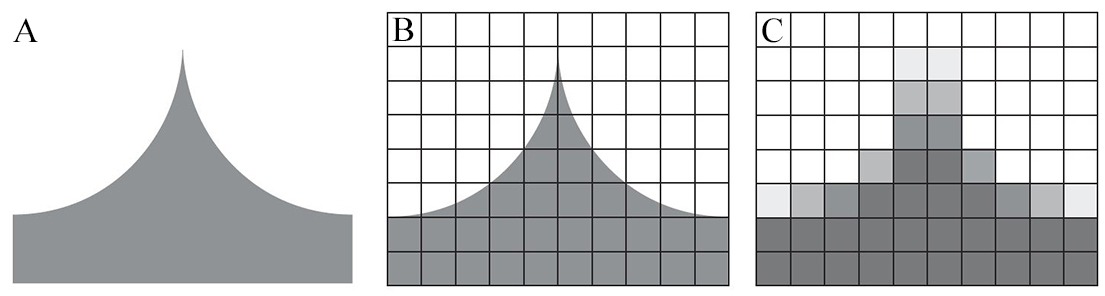
\includegraphics [width = 0.7\textwidth, height =\textheight, keepaspectratio]{black_partial_pixel}
    \caption{Illustration of the partial pixel effect: \textbf{A}: shows the actual shape of the object; \textbf{B}: shows the pixel grid applied to the original shape; \textbf{C} shows the partial pixel effect, where each pixel receives a gray scale according to the average density of the pixel, causing loss of detail. From Bibbs et al \parencite{Reference1}}
    \label{fig: black_partial_pixel}
\vspace{-10pt}
\end{figure}
\\

In optical scans, a frequent problem is the presence of \emph{\textbf{noise}} on the surface of the scan. This is due to various causes, but this problem can be solved with algorithms that calculate the average of the curvature of the surface and remove the points that deviate from it (the variance in the distribution of points is often an adjustable parameter in the cleaning algorithm ).

\begin{figure}[h]
    \centering
    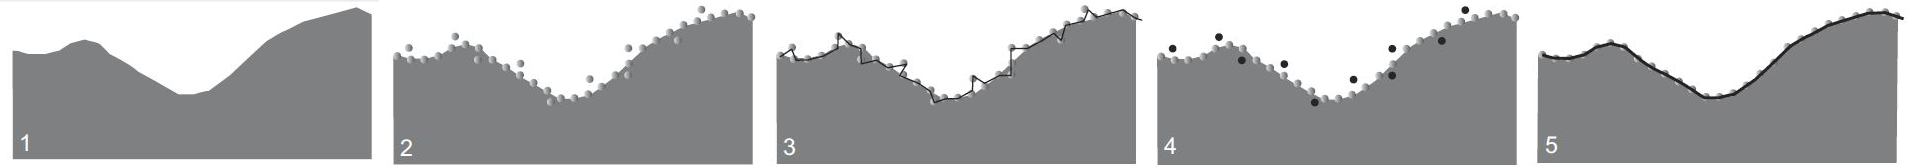
\includegraphics[width=\textwidth, height=\textheight, keepaspectratio]{orizontal_noise}
    \caption{(1) shows the original morphology of the object. (2) shows the reconstruction obtained from the scan. (3) shows the evaluation of the homogeneity of the scan surface. (4) shows the selected points that deviate from the average position of the points on the surface. (5) clean scan (\emph{denoising}). Modified From Bibbs et al \parencite{Reference1}.}
    \label{fig:orizontal_noise}
\end{figure}

\section{The safety of medical images}
DICOM files contain sensitive patient data, such as general information, medical history and diseases, as well as medical images. These files are often sent to colleagues for advice, shared for research purposes or shown to students during teaching. There are online libraries where diagnostic image sets are loaded for research purposes, and these are freely accessible on the web \parencite{Reference24}. To allow a more secure management of images preserving the possibility of sharing, several methods have been proposed. \\
Essential is the protection of patient data in the network in which the data is collected. Computers and servers should be protected by a firewall, while data should only be sent via a VPN. But this is not enough to protect the data when they as to leave the original network. This is why the data must be anonymized or encrypted.

\subsection{Anonymization}
Anonymization consists of removing entries containing sensitive data from the DICOM file. However, the right balance between the data removed for security and those to be maintained must be found, because items such as date of birth, sex and date of execution of the surveys are important both in the subsequent study of the images and for their management.\\
Anonymization is not always necessary if images are to be kept in a private and protected archive, but should be used when the file is spread and there is a risk to the patient's privacy. \\
Several software, open-source or commercial, have been proposed for the scope, for example DICOM Confidential \parencite{Reference46}. \\Anonymisation is an \textbf{irreversible} process, because is impossible to retrieve data after that they have been removed from the DICOM file.

\subsection{Encryption}
Encryption is essentially the process of translating data into another form to prevent them from being easily understood. \\ Replacing every letter of a word with the following letter in the alphabet (hello -> dlbp) is an example of \emph{symmetric key cryptography}, because the key (replacing every letter of the message with the next to encrypt and with the previous one to decipher) is the same for both parties that exchange the message. The \emph{asymmetric key algorithms} work with a key for encryption (\emph{public key}) and a key for decryption (\emph{private key}). \\ \textbf{RSA} is an asymmetric key algorithm, whereas \textbf{AES} is a symmetric key algorithm; both are supported by the DICOM Standard. The choice of the algorithm must however be made not only looking at security, but also at the time of encryption-decryption. RSA is currently considered very safe, but it is also slower to calculate; for this reason RSA is used to generate keys, which is a process that is performed infrequently, while AES is used with RSA keys to encode data \parencite{Reference25}. \\
Encryption is a completely \textbf{reversible} process, so there is no loss of data during the process.

\subsection{Evaluation of data integrity}
There are many ways to exchange data, and this flexibility comes at the risk that the data is somehow changed without permission. To solve this problem we can use another tool borrowed from cryptography: \emph{\textbf{hash function}}. The hash function is essentially an algorithm that takes as \emph{input} an arbitrary sequence of bits, and give as \emph{output} a standard sequence of bit. When the input is changed, there is a very high probability that the output will change. \\
If, for example, in a CT the value of one or more pixels is changed, or the date of acquisition is changed, when the hash is assessed the output will not match the original one, which indicates that given is corrupted. \\
QuickHash GUI is a cross-platform open-source software with a graphical interface, which allows to create hash of files and folders and to check their authenticity \parencite{Reference65}.
\begin{figure}[h]
    \centering
    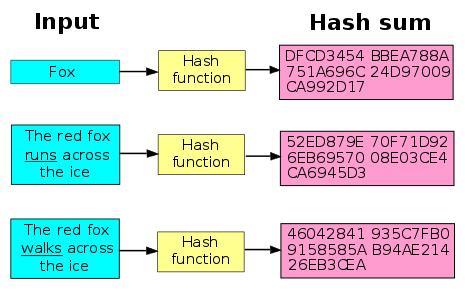
\includegraphics [width=0.6\textwidth, height=\textheight, keepaspectratio]{Hash_function}
    \caption {scheme of a hash function: an input is processed with a hash function, which results in a standardized output. From \emph{Wikipedia}}
    \label{fig:Hash_function}
\end{figure}

\subsection{Evaluating data source}
When two operators exchange data, who receives the data must be sure of the validity of the sender.
With digital data, this confirmation is given by the digital signature. The digital signature is a sequence of characters that is issued by trustworthy entities after ascertaining the credentials of the applicant. The recipient of the data will then be able to discriminate the valid sender based on his signature.

